\section{弱衰变与壳演化的互补探针}\label{sec:4-7}

在第2.2节中，我们阐明了单极相互作用与张量力驱动单粒子轨道漂移的壳演化微观机制；在第2.3节与第2.7节中，分别确立了 BCS 准粒子配对表象以及截断模型空间中有效电磁与弱跃迁算符的重整化规范；在第4.6节中，推演了同核异能态对多体波函数特定微观对称性与几何取向的选择定则。然而，电磁衰变与同核异能跃迁本质上属于同核内部不同激发态之间的电荷与电流响应，其质子数与中子数严格保持守恒。与此截然不同，弱相互作用 $\beta$ 衰变直接改变核内的质中比（$Z \to Z \pm 1$），能够在整条同量异位素链上横向探测单粒子波函数的占据几率、费米面附近的泡利阻塞效应以及集体运动自由度的微观重组。

这便引出了本节需要回答的核心问题：\textbf{弱相互作用衰变在何种机制下充当了原子核壳层演化、形状形变与超流配对的灵敏互补探针？实验观测到的有限衰变能窗、缓发粒子发射与双贝塔衰变矩阵元，如何对微观多体波函数施加严格的物理约束？}

本节划分为三个循序渐进的子模块：
\begin{enumerate}
\item \textbf{4.7.1节：Gamow-Teller、一阶禁戒与有限 Q 衰变能窗。} 将全 Hilbert 空间的几何代数和定则与实际有限能窗内的实测衰变速率严格区分，剖析原子核形变、轨道占据与粒子-振动耦合对跃迁强度的重分配与解阻塞效应，推演微分衰变能谱并界定守恒矢量流（CVC）的适用边界；
\item \textbf{4.7.2节：逐态 $\beta$ 缓发级联与中子多重度。} 阐述 $\beta$ 衰变前向馈送后高激发态在 $\gamma$ 辐射退激与中子发射之间的非相干统计级联竞争，给出发射几率的吸收级联概率分解，辨析不同文献中 $P_{1n}$、$P_{\ge 1n}$ 与平均多重度 $\langle M_n \rangle$ 的物理定义，纠正将 $Q_\beta - S_n$ 单纯当作充分预测公式的认识误区；
\item \textbf{4.7.3节：形变、配对与轻中微子 $0\nu\beta\beta$ 矩阵元范围。} 聚焦标准轻 Majorana 中微子交换机制，对比低能单 $\beta$ 衰变与双贝塔衰变在特征虚动量转移上的本质差异，阐述手征有效场论中 $\Delta L = 2$ 短程接触算符的重整化自洽性，剖析配对相干与四极形变错位对核矩阵元的调制作用。
\end{enumerate}

\subsection{Gamow-Teller、一阶禁戒与有限 Q 衰变能窗}\label{sec:4-7-1}

在第2.7节中，我们推导了完备状态空间中的裸单体 Gamow-Teller 算符与 Ikeda 差和定则：在 $t_3(n) = +1/2$、$t_3(p) = -1/2$ 与 $t_- |n\rangle = |p\rangle$（即 $\beta^-$ 跃迁降低核系统总同位旋第三分量 $T_3 = (N - Z)/2$）约定下，总跃迁强度定义为对所有可达末态的约化跃迁几率求和 $S_\mp \equiv \sum_{f_\mp} B(GT^\mp; J_i \to J_f) = \frac{1}{2J_i + 1} \sum_{f_\mp} |\langle f_\mp \| \sum_k \boldsymbol{\sigma}(k) t_\mp(k) \| J_i \rangle|^2$（约化跃迁几率 $B(GT^\pm)$ 的标准定义已包含初态自旋统计平均因子 $1/(2J_i + 1)$），由同位旋换位子 $[t_+, t_-] = 2 t_3$ 与全 Hilbert 空间完备闭合性给出 $S_- - S_+ = 3(N - Z)$。该定则是基于裸算符在无截断空间中导出的纯空间-同位旋几何代数恒等式，其裸定义本身完全独立于外在弱耦合常数 $g_A$ 及轻子运动学相空间加权。若引入常数有效淬灭因子 $q \equiv g_A^{\mathrm{eff}} / g_A^{\mathrm{bare}}$ 对单体 GT 矩阵元进行全局缩放，则差和相应按 $q^2$ 缩放为 $3 q^2 (N - Z)$；而在截断价空间（如准粒子 RPA 模型空间）中，差和定则的严格满足依赖于自旋-轨道劈裂伙伴轨道是否完全包含在模型空间内，且两体弱介子交换流（2BC）的引入将通过额外的微观代数项修正简单的单体求和。

在真实放射性衰变测量中，物理衰变速率严格受限于有限的衰变能释放窗（$Q$ 值）。采用中性基态原子质量 $M(A,Z)$，并暂略原子反冲与微小质量修正，有
\begin{align}
Q_{\beta^-}&=[M(A,Z)-M(A,Z+1)]c^2,\label{eq:4-7-Q-betaminus}\\
Q_{\beta^+}&=[M(A,Z)-M(A,Z-1)-2m_e]c^2,\label{eq:4-7-Q-betaplus}\\
Q_{\mathrm{EC}}&=[M(A,Z)-M(A,Z-1)]c^2.\label{eq:4-7-Q-EC}
\end{align}
前两式分别是 $\beta^-$、$\beta^+$ 的可用动能；$\beta^+$ 的开放条件为 $Q_{\beta^+}>0$。对捕获电子壳层 $j$、布居核激发能 $E_x$ 的分支，最终原子具有相应空穴，近似产生能量
\begin{equation}\label{eq:4-7-Q-EC-neutrino}
E_\nu(j,E_x)=Q_{\mathrm{EC}}-E_x-B_j
\end{equation}
的单色中微子；这里 $B_j$ 取子核对应的中性原子基态中该壳层电子的结合能。在运动学上，$\beta^-$ 衰变出射反中微子 $\bar{\nu}_e$，而 $\beta^+$ 衰变与电子俘获（EC）出射中微子 $\nu_e$；二者不可混写，亦不可将 $\beta^+$ 的 $-2m_e c^2$ 阈值套用到电子俘获之上。

根据弱相互作用有效拉氏量理论，出射带电轻子（动量为 $p_e$、总能量为 $E_e$）的微分发射速率公式写作：
\begin{equation}\label{eq:4-7-differential-spectrum}
\frac{d\lambda}{dW} = \frac{(G_F^{(E)})^2 |V_{ud}|^2 (m_e c^2)^5}{2\pi^3 \hbar} F(Z, W) p W (W_0 - W)^2 C(W),
\end{equation}
这里 $G_F^{(E)}$ 是自然单位制中以 $\mathrm{MeV}^{-2}$ 表示的费米常数，约为 $1.16638\times10^{-11}\,\mathrm{MeV}^{-2}$。式中 $m_e c^2$ 用能量单位，$\hbar$ 用能量乘时间单位，故前因子量纲为 $\mathrm{s}^{-1}$。若另用量纲为能量乘体积的 $G_F^{(\mathrm{SI})}$，才有 $G_F^{(E)}=G_F^{(\mathrm{SI})}/(\hbar c)^3$；不得对已用 $\mathrm{MeV}^{-2}$ 表示的常数再次除以 $(\hbar c)^3$。各运动学变量均以电子静止能量 $m_e c^2$ 无量纲化：
\begin{itemize}
\item $W \equiv 1 + \frac{T_e}{m_e c^2} = \frac{E_e}{m_e c^2}$ 为轻子无量纲总能量（$T_e$ 为轻子动能，$W \ge 1$）；
\item $p \equiv \frac{p_e c}{m_e c^2} = \sqrt{W^2 - 1}$ 为无量纲轻子动量；
\item $W_0 \equiv 1 + \frac{Q_\beta - E_x}{m_e c^2}$ 为对应于子核激发能为 $E_x$ 的特定退激分支的无量纲最大端点能量；
\item $F(Z, W)$ 为相对论 Fermi 函数，描述子核库仑势场对出射轻子波函数的连续态畸变（子核电荷取 $Z_{\mathrm{final}}$，对 $\beta^-$ 表现为库仑吸引 $F > 1$，对 $\beta^+$ 表现为库仑排斥且在低能端受阻遏）；
\item $C(W)$ 为谱形状因子（Shape Factor）。在无轨道角动量转移（$\Delta L = 0$）的允许跃迁中，若略去核子反冲修正、诱导流以及轻子波函数在核体积内的微小径向变化，形状因子可近似视为与能量无关的常数：
\begin{equation}\label{eq:4-7-shape-factor-allowed}
C_{\mathrm{allowed}}(W) \approx g_V^2 B(F) + g_A^2 B(GT),
\end{equation}
其中
\[
\begin{aligned}
 B(F)&=\frac{|\langle f\|\sum_k t_\pm(k)\|i\rangle|^2}{2J_i+1},\\
 B(GT)&=\frac{|\langle f\|\sum_k\boldsymbol\sigma(k)t_\pm(k)\|i\rangle|^2}{2J_i+1}.
\end{aligned}
\]
二者均采用单粒子同位旋算符 $t_\pm$（沿用第~2.7~节约定，且不含 $g_V$ 或 $g_A$），因而式~\eqref{eq:4-7-shape-factor-allowed} 中弱耦合常数只计一次。式~\eqref{eq:4-7-differential-spectrum} 为所述允许近似下的最低阶展开写法；弱电辐射修正（$\delta_R$）、核有限尺寸效应与非零核子反冲修正需按所采用的精度框架显式计入。在上述最低阶无量纲化约定下，式中的 Fermi 函数 $F(Z, W)$ 与形状因子 $C(W)$ 均为无量纲量；未加辐射修正的前因子常数 $K_0 \equiv \frac{2\pi^3 \hbar \ln 2}{(G_F^{(E)})^2 |V_{ud}|^2 (m_e c^2)^5} \approx 6292\,\mathrm{s}$（取 $G_F^{(E)} = 1.16638 \times 10^{-11}\,\mathrm{MeV}^{-2}$，$|V_{ud}| = 0.974$），与 Zhi 等采用的参考常数 $K = 6146\,\mathrm{s}$（如 Zhi 等~\cite{doctoral-r1-g34-zhi-2013-prc-shell-model-half-lives} 所用，其 Eq.(2) 给出了相应的相空间积分定义）有数值差异；比较时须核对弱耦合、辐射修正和强度定义，不能仅由此差值反推原文的修正组成。若引用已把 $(g_A/g_V)^2$ 吸收入 $B(GT)$ 的文献资料，亦应统一换算，不可重复乘入相同因子。此式针对指定 $\beta^\mp$ 分支；EC 应采用束缚电子波函数和离散中微子能量，不能直接套用连续 $\beta$ 谱。对能量积分得到的标准 Fermi 相空间因子 $f_0(Z, W_0) = \int_1^{W_0} F(Z, W) p W (W_0 - W)^2 dW$，其呈现的 $f_0 \propto Q_\beta^5$ 标度仅在超相对论与无库仑极限（$Z \to 0, W_0 \gg 1$）下成立，并非在全能量与全电荷区普遍精确的幂次。
\end{itemize}

在此需要澄清\textbf{守恒矢量流假设（CVC 假说）的微观适用范围}。CVC 假说断言弱矢量流与电磁同位旋流构成同一同位旋三态矢量，因此在同位旋对称性极限下，全空间积分配对的零动量总矢量荷算符 $\hat{T}_\pm = \int V_0^\pm d^3r$ 在核介质中不发生微观重整化。对于同位旋多重态之间的 Fermi 超允许跃迁，其矩阵元由同位旋升降算符代数严格给出：
\begin{equation}\label{eq:4-7-fermi-matrix-element}
\langle T, T_z \pm 1 | \hat{T}_\pm | T, T_z \rangle = \sqrt{T(T+1) - T_z(T_z \pm 1)}.
\end{equation}
文献中常见的 $\sqrt{2}$ 因子仅对应于 $T=1$ 同位旋三态（$T=1, T_z = \mp 1 \to T_z = 0$，如 $0^+ \to 0^+$ 超允许衰变）的特殊取值，不能直接推广到一般多重态。更重要的是，\textbf{CVC 假说对弱矢量流的保护严格体现在流守恒的场论微分恒等式中}：在零动量转移极限下，该守恒性确保了总时间分量弱矢量荷矩阵元不受强相互作用强重整化（$g_V = 1$）；而在有限动量转移下，CVC 假说进一步提供了空间矢量流与特定禁戒跃迁形状因子之间的微观代数联系（例如 Zhi 等~\cite{doctoral-r1-g34-zhi-2013-prc-shell-model-half-lives} 中依据 CVC 导出的矢量核矩阵元之间的一致性比例关系），但 CVC 并不能对弱轴矢量流提供相同的守恒保护。在有限动量转移、截断模型空间有效算符重整化以及库仑同位旋破缺效应下，弱矢量流矩阵元依然包含非平庸修正，不可将 CVC 误解为所有弱相互作用跃迁在核介质中均不受有效重整化。

在实际原子核能谱中，微观壳演化、形变与配对关联深刻调控着 Gamow-Teller 强度的能量分布：
\begin{enumerate}
\item \textbf{激发能级拓扑与有限能窗截断：} 在球形双闭壳核附近，很大一部分 Gamow-Teller 跃迁强度相干聚集在巨共振峰（GTGR）中。当 $Q_\beta$ 能窗显著低于巨共振能量时，衰变仅能布居其低能尾部，实测衰变速率直接受制于低能态的组态波包，不能单纯依据 $3(N-Z)$ 预测实际半衰期。
\item \textbf{四极形变与 Nilsson 轨道劈裂：} 原子核产生四极形变时，球形单粒子多重态劈裂为若干具有不同角动量投影 $\Omega$ 的 Nilsson 能级。这种单粒子谱的展宽使原本局域在高能区的 GT 强度发生碎裂并重构其能谱拓扑；形变引起的能级移动可对低能 $Q_\beta$ 衰变能窗内的强度产生重分配，其移动方向与强弱取决于费米面附近的具体单粒子轨道排布与组态结构，进而改变原子核的弱衰变半衰期。
\item \textbf{粒子-振动耦合（PVC）与多体强度的重分配：} 在纯单粒子壳模型或静态 RPA 计算中，若母核中子与子核质子的单粒子能级排布受到泡利不相容原理强烈阻遏，模型可能预言衰变能窗内的低能 GT 强度严格为零或极度微弱。然而正如 Wang 等在双闭壳核 $^{56}\mathrm{Ni}$、$^{100}\mathrm{Sn}$ 与 $^{132}\mathrm{Sn}$ 中的微观 RPA 与 PVC 联合计算所示~\cite{wang-2026-axial-coupling-quenching-joint-effects}，多粒子-多空穴关联与核芯表面振动声子相互作用对低能强度的重分布具有高度特异性：在自共轭核 $^{56}\mathrm{Ni}$ 中（涉及电子俘获衰变通道），引入 PVC 确实打破了闭壳冻结，在原本零强度的低能区产生微弱的解阻塞（Unblocking）强度；但在极丰中子双闭壳核 $^{132}\mathrm{Sn}$ 中，即便计入 PVC，采用 SGII Skyrme 相互作用在其实验物理 $Q_\beta$ 能窗内依然预言零 GT 强度（仅在 SkM* 参数下产生拖入能窗的微弱低能尾部），其实际半衰期仍主要受一阶禁戒跃迁主导。这表明微观多体关联不仅有淬灭效应，亦能引起强度的拓扑重分配，但不可将解阻塞效应过度推论为在所有双闭壳核中均普遍成立的开通机制。
\end{enumerate}

在远离稳定线的快中子俘获过程（$r$-过程）等待点核区，允许 Gamow-Teller 跃迁与一阶禁戒跃迁（First-Forbidden, FF，$\Delta \pi = -1$）的相对重要性随质量区发生显著演化。依据 Zhi 等人基于大尺度壳模型跨壳层计算的系统分析~\cite{doctoral-r1-g34-zhi-2013-prc-shell-model-half-lives}：
\begin{itemize}
\item 在 $N=50$（$Z \ge 28$，包括 $^{78}\mathrm{Ni}$）与 $N=82$（如 $^{130}\mathrm{Cd}$）等待点核区，Gamow-Teller 衰变仍然是主导衰变模式。例如在 $^{130}\mathrm{Cd}$ 中，计算证实 GT 衰变贡献了主导份额（采用有效淬灭因子 $q(GT) = 0.66$），一阶禁戒跃迁对计算半衰期的缩短贡献仅约 $13\%$；而在 $^{78}\mathrm{Ni}$ 中，独立粒子模型下中子 $1g_{9/2} \to \text{质子 } 1f_{7/2}$ 的 rank-1 FF 跃迁受到泡利阻塞，多体组态混合虽部分解除了这一阻塞，但在 $N=50$ 同中子素中 FF 贡献总体依然微弱（通常低于 $5\%$）。
\item 在 Zhi 等所研究的 $N=126$ 壳模型核素中，随质子数增加，GT 道因相关轨道的泡利阻塞而减弱；对于所算 $Z \ge 70$ 核素，FF 对半衰期的贡献超过 GT。这是该模型与核素范围内的结果，不是所有 $N=126$ 核素的普适结论。
\end{itemize}
以下只示意一阶禁戒算符的张量秩与宇称结构，动量写法取 $c=1$；实际数值计算需沿同一来源使用径向尺度和系数，不将不同量纲的示意算符直接相加。非相对论约化后包含的结构~\cite{doctoral-r1-g34-zhi-2013-prc-shell-model-half-lives}：
\begin{itemize}
\item 秩为 0 的类时轴荷算符：$\hat{\mathcal{O}}_0 \propto \gamma_5 \to \frac{\boldsymbol{\sigma} \cdot \mathbf{p}}{m_N}$，还包括 $[\mathbf r\otimes\boldsymbol\sigma]^{(0)}$ 型自旋偶极结构；
\item 秩为1的空间矢量与轴矢量结构：$\hat{\mathcal{O}}_1 \propto \mathbf{r}, \boldsymbol{\alpha} \to \frac{\mathbf{p}}{m_N}, \boldsymbol{\sigma}\times\mathbf{r}$；
\item 秩为 2 的空间张量算符：$\hat{\mathcal{O}}_2 \propto [\boldsymbol{\sigma} \times \mathbf{r}]_2$。
\end{itemize}
Zhi 等人在微观壳模型中表明：软 $\pi$ 介子交换流使类时轴荷算符表现出介质增强（拟合有效参数 $q(\xi' v) = 1.266 > 1$），而空间分量算符则呈现出不同程度的淬灭（秩 1 矢量算符 $q(x) = 0.51$，秩 1 轴矢量算符 $q(u) = 0.38$，秩 0 轴矢量算符 $q(w) = 0.66$，秩 2 张量算符 $q(z) = 0.42$）~\cite{doctoral-r1-g34-zhi-2013-prc-shell-model-half-lives}。对未极化初态、末态磁量子数未观测且轻子角度已积分的微分能谱，式~\eqref{eq:4-7-differential-spectrum} 中的形状因子 $C(W)$ 依赖电子能量，各核张量秩的贡献分块相加；同秩内不同算符矩阵元可相干干涉，例如秩 1 的 $x$ 与 $u$。这一结论限于上述能谱，不排除极化或角关联观测量中的其他干涉；单一标量淬灭因子仍不能简单推广至所有禁戒通道。

\subsection{逐态 $\beta$ 缓发级联与中子多重度}\label{sec:4-7-2}

当原子核极度偏离稳定线走向极丰中子区时，核质量差 $Q_\beta$ 显著升高，而子核的中子分离能 $S_n$（以及多中子分离阈值 $S_{2n}, S_{3n}$）则因过剩中子结合减弱而降低。当满足动学条件 $Q_\beta > S_n$ 时，母核通过 $\beta$ 衰变能够布居到子核中子分离阈值之上的激发态。这些处于非束缚连续谱中的激发能级随后迅速退激，产生 \textbf{$\beta$ 缓发中子发射（$\beta$-delayed neutron emission）}~\cite{dimitriou-2021-iaea-beta-delayed-neutron-database}。

在弱布居与后续退激可分离、各步能用非负部分宽度描述且相干干涉可忽略的近似下，$\beta$ 缓发粒子发射可以表示为两阶段的条件概率模型：
\begin{enumerate}
\item \textbf{弱馈送：} 令 $I_\beta(i)$ 为每次母核总衰变中直接馈送子核激发态 $i$ 的无量纲概率，离散态求和并包含连续谱积分后满足母核衰变分支比归一：
\begin{equation}\label{eq:4-7-beta-feeding-normalization}
\sum_i I_\beta(i) = b_\beta \le 1.
\end{equation}
若母核还存在自发裂变、$\alpha$ 衰变或结团发射等竞争道，则 $\beta$ 衰变分支比 $b_\beta < 1$。
\item \textbf{级联退激与吸收马尔可夫链：} 子核处于激发能高于中子分离阈的状态时，通过中子发射与辐射 $\gamma$ 级联竞争退激。令 $\Pi_x(a)$ 为处于激发态 $a$ 的体系经过相继退激级联最终总共释放 $x$ 个中子的净吸收概率。对于任意非终止的瞬态能级 $a$，$\Pi_x(a)$ 满足离散差分递推关系：
\begin{equation}\label{eq:4-7-cascade-pi-def}
\Pi_x(a) = \sum_{b, r} \frac{\Gamma^{(r)}_{a \to b}}{\Gamma_{\mathrm{tot}}(a)} \Pi_{x-r}(b), \qquad \Pi_{x < 0}(a) \equiv 0,
\end{equation}
其中 $\Gamma^{(r)}_{a \to b}$ 为从状态 $a$ 释放 $r$ 个中子（$r = 0, 1, 2, \dots$）跃迁至状态 $b$ 的部分衰变宽度，$\Gamma_{\mathrm{tot}}(a)$ 为该态全部开放通道的总退激宽度。对于被选定为终止退激的吸收态 $t$（如在所选观测时窗内不再释放中子的子核束缚基态或长寿命同核异能态），满足边界条件 $\Pi_x(t) = \delta_{x0}$。当所列通道在选定时窗内几乎必然完全吸收时，全多重度概率守恒 $\sum_{x \ge 0} \Pi_x(a) = 1$。

按每次母核总衰变归一的 $\beta$ 缓发 $x$ 中子发射净分支比，以及按 $\beta$ 衰变事件条件归一的中子发射几率分别定义为：
\begin{equation}\label{eq:4-7-conditional-probability}
P_{xn}^{(\beta;\mathrm{parent})} = \sum_i I_\beta(i) \Pi_x(i), \qquad P_{xn}^{(\beta \mid \beta)} = \frac{P_{xn}^{(\beta;\mathrm{parent})}}{b_\beta} \quad (b_\beta > 0).
\end{equation}
前者对所有发射中子数求和等于母核 $\beta$ 衰变分支比 $\sum_{x \ge 0} P_{xn}^{(\beta;\mathrm{parent})} = b_\beta \le 1$，后者则满足条件全概归一 $\sum_{x \ge 0} P_{xn}^{(\beta \mid \beta)} = 1$。
\end{enumerate}
仅在略去多步相继发射（$r \le 1$）且假定阈上 $\gamma$ 衰变全部直达束缚态（$\Pi_1(\text{束缚}) = 0$）的极简单步极限下，能级 $i$ 的发射吸收概率才退化为单步分支比 $\Pi_1(i) \approx \frac{\Gamma_n(i)}{\Gamma_{\mathrm{tot}}(i)}$。

\begin{figure}[!htbp]
\centering
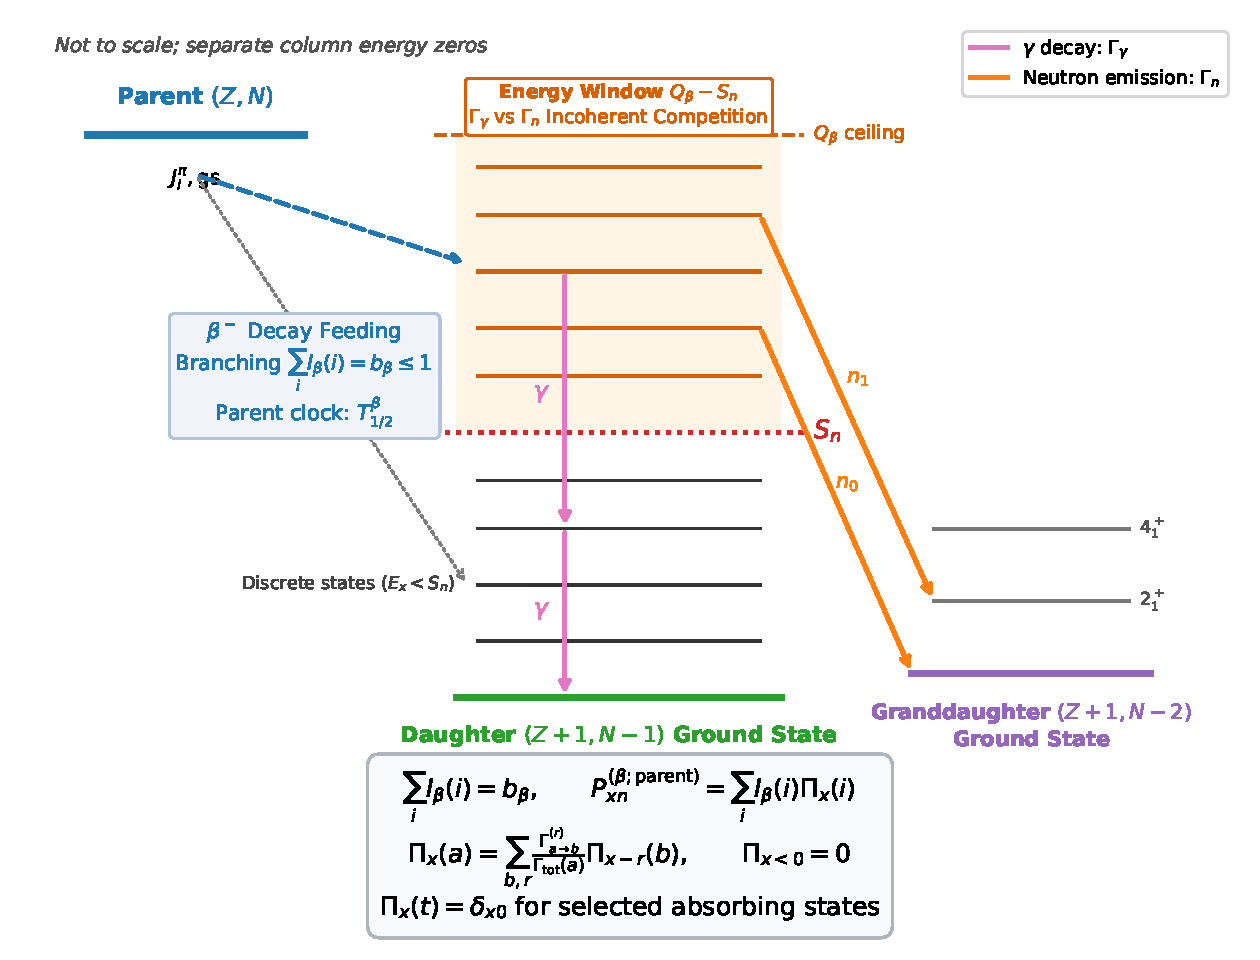
\includegraphics[width=0.98\textwidth]{Img/weak-cascade-competition.pdf}
\caption[前驱母核 $(Z, N)$ 经 $\beta^-$ 衰变馈送至子核 $(Z+1, N-1)$ 高激发态后，在能量窗口 $Q_\beta - S_n$ 内中子发射通道与辐射退激通道的非相干统计级联竞争示意图]{前驱母核 $(Z, N)$ 经 $\beta^-$ 衰变馈送至子核 $(Z+1, N-1)$ 高激发态后，在能量窗口 $Q_\beta - S_n$ 内中子发射通道与辐射退激通道的非相干统计级联竞争示意图（教学原理模型，展示衰变母态分支比归一与级联退激吸收网络，非特定实验装置原始计数）。}\label{fig:weak-cascade-competition}
\end{figure}

式~\eqref{eq:4-7-conditional-probability} 与图~\ref{fig:weak-cascade-competition} 澄清了理论分析中的一个\textbf{关键认识误区}：
\begin{quote}
\textbf{$Q_{\beta n}\equiv Q_\beta-S_n$ 给出单中子通道的可用能量窗口；它本身并不能充分预测中子发射几率 $P_n$。}
\end{quote}
即便子核能级位于中子分离阈值之上（$E_x(i) > S_n$），发射中子也并不具有绝对的必然性。如果激发能仅仅略微高出 $S_n$（出射中子能量极低），而由于初态能级与孙核低激发态之间的自旋宇称匹配要求中子必须携带较高的轨道角动量（如 $l=2$ 或 $l=3$），出射中子波函数将遭受离心势垒（Centrifugal Barrier $V_l = \frac{\hbar^2 l(l+1)}{2\mu r^2}$）的显著阻碍，导致中子发射受到明显抑制。此时，辐射 $\gamma$ 衰变仍然能够有效竞争，使核退激回到子核的束缚基态。此外，当跨越壳层闭合点时，单粒子能隙突变会导致 $Q_\beta$ 与 $S_n$ 发生阶跃式变化，使实际测量的中子发射概率呈现出非连续突变。

在核数据评估与实验测量中，必须严格区分国际原子能机构（IAEA）参考数据库所规范的不同物理定义~\cite{dimitriou-2021-iaea-beta-delayed-neutron-database}：
\begin{enumerate}
\item \textbf{单中子发射几率 $P_{1n}$：} 每次前驱母核总衰变中，恰好释放 1 个中子的净分支几率：
\begin{equation}\label{eq:4-7-P1n-def}
P_{1n}^{(\beta;\mathrm{parent})} = \sum_{i} I_\beta(i) \Pi_1(i);
\end{equation}
\item \textbf{全缓发中子发射总几率 $P_{\ge 1n}$（文献中常通称 $P_n$）：} 每次母核衰变发射至少 1 个中子的总几率：
\begin{equation}\label{eq:4-7-P-atleast-1n-def}
P_{\ge 1n}^{(\beta;\mathrm{parent})} = \sum_{x \ge 1} P_{xn}^{(\beta;\mathrm{parent})} = P_{1n}^{(\beta;\mathrm{parent})} + P_{2n}^{(\beta;\mathrm{parent})} + \dots;
\end{equation}
\item \textbf{平均缓发中子多重度 $\langle M_n \rangle$：} 每次母核衰变平均释放的中子数目：
\begin{equation}\label{eq:4-7-mean-multiplicity-def}
\langle M_n \rangle^{(\beta;\mathrm{parent})} = \sum_{x \ge 1} x P_{xn}^{(\beta;\mathrm{parent})} = P_{1n}^{(\beta;\mathrm{parent})} + 2 P_{2n}^{(\beta;\mathrm{parent})} + 3 P_{3n}^{(\beta;\mathrm{parent})} + \dots.
\end{equation}
\end{enumerate}
当多中子发射道闭合时（$Q_\beta < S_{2n}$），$P_{1n}^{(\beta;\mathrm{parent})} = P_{\ge 1n}^{(\beta;\mathrm{parent})} = \langle M_n \rangle^{(\beta;\mathrm{parent})}$；但在极丰中子核区，$P_{2n}$ 与 $P_{3n}$ 通道开启，三者的数值产生系统性偏离，数据分析时必须根据具体实验观测量进行精确映射。若研究按 $\beta$ 事件条件归一的中子几率，只需将上述各式除以母核分支比 $b_\beta$。

在这里采用的快退激近似下，缓发中子的主要延迟跟随前驱母核的弱衰变时钟；随后子核的中子发射与辐射竞争通过前述级联宽度处理。若某条通道存在不可忽略的额外延迟，应将其纳入时间演化，不能仍把全部时间分布归给母核。中子的飞行、热化和探测器俘获响应则属于另外的测量时间卷积。

设 $R_{y|x}$ 为真实发射 $x$ 个中子后探测系统记录到 $y$ 个信号的条件概率响应矩阵，则无门控母衰变观测到的中子多重度分布满足 $p_y^{\mathrm{obs}} = \sum_x R_{y|x} P_{xn}^{(\beta;\mathrm{parent})} + p_y^{\mathrm{non\text{-}}\beta}$。若母核同时存在自发裂变或带电粒子发射等竞争道，必须将其独立的中子多重度分布与探测器响应单独计入 $p_y^{\mathrm{non\text{-}}\beta}$ 项中，不可将非 $\beta$ 产中子道混同为 $\beta$ 缓发中子，亦不可将所有非 $\beta$ 衰变默认归入 $x=0$ 无中子模式。在理想单粒子效率 $\epsilon_n$、无串扰且忽略多重偶然计数的二项响应近似下，$R_{y|x} = \binom{x}{y} \epsilon_n^y (1 - \epsilon_n)^{x-y}$。实际测量中探测效率显著依赖于出射中子连续能谱、角分布与探测时间关联门，必须通过精准的源标定与 Monte Carlo 输运模拟构建响应矩阵，并通过贝叶斯前向似然或统计非折叠（Unfolding）算法提取真实发射多重度。

\subsection{形变、配对与轻中微子 $0\nu\beta\beta$ 矩阵元范围}\label{sec:4-7-3}

若确认 $0\nu\beta\beta$，在通常局域量子场论框架下将表明轻子数不守恒（$\Delta L = 2$），并通过 Schechter-Valle 黑盒论证确立中微子具有非零 Majorana 质量项；单凭衰变寿命观测本身不能独立证明轻中微子质量机制必定压倒重轻子或超对称等竞争机制，亦不能脱离微观核矩阵元唯象反演有效 Majorana 质量。在标准轻 Majorana 中微子交换占主导的理论假设下，物理过程由核内两个弱流顶点之间交换一条虚中微子传播子所驱动，理论半衰期可写作如下相容的因式分解形式：
\begin{equation}\label{eq:4-7-0nubb-halflife}
[T_{1/2}^{0\nu}]^{-1} = G_{0\nu} g_A^4 |M_{0\nu}|^2 \left|\frac{m_{\beta\beta}}{m_e}\right|^2, \qquad m_{\beta\beta} \equiv \left| \sum_j U_{ej}^2 m_j \right|.
\end{equation}
式中相空间因子 $G_{0\nu}$（以 $\mathrm{yr}^{-1}$ 为单位）按本式定义为已外提无量纲轴矢量常数因子 $g_A^4$；有效质量 $m_{\beta\beta}$ 与电子质量 $m_e$ 采用相同的质量或静止能量单位（使质量比无量纲）；微观核矩阵元 $M_{0\nu}$ 的多极展开、核子电弱形状因子、有限核半径 $R = 1.2 A^{1/3}\,\mathrm{fm}$ 标度规范必须与相空间因子 $G_{0\nu}$ 保持严格相容~\cite{engel-menendez-2017-double-beta-matrix-elements-review}。若文献定义吸收了耦合因子的相空间 $\widetilde{G}_{0\nu} \equiv G_{0\nu} g_A^4$，则外部不可重复乘入 $g_A^4$。
传统长程部分可写成
\begin{equation}\label{eq:4-7-NME-decomposition}
M_{0\nu}^{\mathrm{long}}=M_{GT}-\left(\frac{g_V}{g_A}\right)^2M_F+M_T.
\end{equation}
该轻中微子单线虚交换在核内涉及宽广的虚拟动量积分谱，其动量转移峰值位于 $|\mathbf{q}| \sim 100\text{--}200\,\mathrm{MeV}/c$（对应核子间距 $r \sim 1\text{--}2\,\mathrm{fm}$），在特征尺度上远远超出了单 $\beta$ 衰变的长波长零动量极限。
Cirigliano 等在基于手征有效场论对两核子 $^1S_0$ 散射非微扰重整化的分析中指出~\cite{cirigliano-2018-leading-short-range-double-beta}：单独的长程单中微子交换势 $V_\nu^{\mathrm{long}} \sim 1/r_{12}$ 会引入依赖于截断尺度的紫外发散；为了在两核子非微扰散射中满足重整化群自洽性，手征领头阶（LO）需引入一个 $\Delta L = 2$ 的两核子短程接触相互作用势。Cirigliano 等在文献中以 $\tau_{1,+} \tau_{2,+}$ 标示 $n n \to p p$ 同位旋跃迁；转换至本节所用的同位旋约定（$t_3(n) = +1/2, t_- |n\rangle = |p\rangle$），在剥离弱耦合与轻子因子后，其在自然单位制与坐标空间中的 $^1S_0$ 剥离相互作用势写作 $V_{\mathrm{CT}}^{(R)}(\mathbf{r}_{12}) = -2 g_\nu^{NN}(R) \delta_R^{(3)}(\mathbf{r}_{12}) t_{1,-} t_{2,-}$。该接触项的有效强度 $g_\nu^{NN}$ 具有正规化方案依赖性；现有文献尝试利用电荷独立性破缺（CIB）电磁数据约束反项低能常数组合（$C_1 + C_2$），但要确定单一耦合 $g_\nu^{NN} = C_1$ 仍需引入额外对称性假设（如 $C_1 \approx C_2$）或与格点 QCD 匹配，不能单凭该电磁数据直接唯一标定。该接触项属于 $\Delta L = 2$ 的双核子超弱通道，与单 $\beta$ 衰变中源自介子交换流的两体轴流（2BC）具有不同的物理机制。

原子核的微观波函数——特别是配对与形变——对 $M_{0\nu}$ 起着关键的调制与选择作用：
\begin{itemize}
\item \textbf{超流配对关联的相干性：} 双贝塔衰变将两个初态配对核子转换为两个末态配对核子。超流 BCS 凝聚态中同位旋矢量（$T=1$）核子对的相干叠加能够有效增大矩阵元；然而，若体系中存在较强的同位旋标量（$T=0$）质中配对竞争，不同配对道之间的干涉反而可能对矩阵元产生削弱效应。
\item \textbf{四极形变错位的微观压制：} 多数候选双贝塔衰变核处于球形到形变的过渡区。若母核与子核在自洽能量曲面上表现出不同的形变极小（例如长椭球母核衰变到扁椭球或弱形变子核），初末态微观内禀波函数在形状坐标空间中将出现波包错位。这种内禀波函数重叠的减弱，会对核矩阵元产生显著的压制效应，其具体压制幅度高度依赖于所选用的微观形变模型。
\item \textbf{反演非唯一性与微观不确定度：} 实验上测量到的双贝塔半衰期下限，是相空间、有效 Majorana 质量、有效轴矢量耦合 $g_A$ 以及多体波函数重叠共同作用的标量结果。从单一的半衰期测量值无法唯一反演局域形变参数或确定的 $g_A$ 淬灭数值，需结合电荷交换反应、双 Gamow-Teller 激发实验以及双核子转移反应等独立手段，对初末态的组态波函数施加协同约束。
\end{itemize}

\subsection{本节小结与微观探针接口}\label{sec:4-7-4}

本节确立了弱相互作用作为低能原子核结构、壳演化与微观关联多维探针的理论图像：
\begin{enumerate}
\item \textbf{有限能窗与强度分布重塑：} 实测 $\beta$ 衰变速率受限于有限能窗 $Q_\beta$ 与微分相空间谱。CVC 假说在零动量转移极限下保证弱矢量荷不受强相互作用强重整化，并在有限动量下约束矢量流，但不保护轴矢量流；四极形变引起 Nilsson 轨道劈裂重构 GT 巨共振分布，而粒子-振动耦合（PVC）在特定闭壳核组态下能够重构低能强度（但在不同核素与相互作用下表现各异，例如 $^{132}\mathrm{Sn}$ 在 SGII 下能窗内仍无 GT 强度）。在 $N=50, 82$ 区 GT 跃迁依然主导；而在 Zhi 等壳模型研究的 $N=126$ 核素中（$Z \ge 70$），随质子数增加 GT 因泡利阻塞减弱，FF 贡献反超 GT（受限于具体模型与核素范围）。
\item \textbf{缓发级联的两阶段统计竞争：} $\beta$ 缓发中子发射遵循条件概率分解式 $P_{xn}^{(\beta;\mathrm{parent})} = \sum_i I_\beta(i) \Pi_x(i)$ 及式~\eqref{eq:4-7-cascade-pi-def} 的逐步计数递推。能量差 $Q_\beta - S_n$ 仅设定理论上限，高于 $S_n$ 的能级仍面临离心势垒阻碍下的辐射 $\gamma$ 竞争退激；必须在定义与测量上严格区分按母核总衰变归一的 $P_{xn}^{(\beta;\mathrm{parent})}$ 与按 $\beta$ 衰变条件归一的 $P_{xn}^{(\beta\mid\beta)}$，以及单中子发射率 $P_{1n}$、全发射率 $P_{\ge 1n}$ 与平均中子多重度 $\langle M_n \rangle$。
\item \textbf{高动量转移下 $0\nu\beta\beta$ 矩阵元特征：} 在本文所述的标准轻 Majorana 中微子交换机制下，衰变由核内两核子弱流顶点之间交换一条虚中微子传播子所驱动，其特征虚动量转移达到 $|\mathbf{q}| \sim 100\text{--}200\text{ MeV}/c$（对应短程 $1\text{--}2\text{ fm}$）；手征有效场论非微扰散射的重整化要求引入领头阶 $\Delta L = 2$ 短程接触算符，其低能常数可借核子--核子散射中的电荷独立性破缺数据约束但不可由该数据单独唯一确定；配对相干与形变错位对核矩阵元产生竞争性调制，不可由单一寿命结果反向推断唯一的形变或淬灭参数。
\end{enumerate}

本节建立的弱衰变理论模型，构筑了以下跨章理论接口：
\begin{itemize}
\item \textbf{对第4.8节（核天体物理反应网络与开放系统演化）：} 极丰中子核素的实际 $\beta$ 衰变半衰期与缓发中子多重度 $\langle M_n \rangle$，与中子俘获/光致蜕变反应率、核质量以及天体环境的温度、中子密度和膨胀时间尺度等动力学参数共同影响着快中子俘获过程（$r$-过程）的反应路径走向与元素丰度峰位置分布；
\item \textbf{对第5章（在束实验谱学技术链）：} 母核的弱衰变时钟与出射中子的飞行、热化及俘获响应属于不同的时间演化环节；在束与放射性束流实验中，全吸收谱仪（TAGS）与中子探测阵列需结合母核衰变周期、能谱特性及时间关联门进行本底抑制与符合测量，并通过构建探测响应矩阵反演真实馈送与多重度分布。
\end{itemize}
